\documentclass[fr]{../../../eplsummary}
\usepackage[french]{varioref} % \vref and \vpageref
\usepackage{graphicx} % images
\usepackage{float} % images
\usepackage{url}
	\urlstyle{sf}
\usepackage[backgroundcolor=yellow]{todonotes} %% todonotes: \listoftodos & \todo{Some note or other.} & \missingfigure{}

% draw
\usepackage{tikz}
\usetikzlibrary{arrows,automata,calc}
\tikzset{
    %Define standard arrow
    >=stealth',
    % Define arrow style
    pil/.style={
           ->,
           thick,
           shorten <=2pt,
           shorten >=2pt,}
}
% \usepackage{qtree}    % dessiner des arbres %% => texlive-humanities

\definecolor{codeBlue}{rgb}{0,0,1}
\definecolor{webred}{rgb}{0.5,0,0}
\definecolor{codeGreen}{rgb}{0,0.5,0}
\definecolor{codeGrey}{rgb}{0.6,0.6,0.6}
\definecolor{webdarkblue}{rgb}{0,0,0.4}
\definecolor{webgreen}{rgb}{0,0.3,0}
\definecolor{webblue}{rgb}{0,0,0.8}
\definecolor{orange}{rgb}{0.7,0.1,0.1}

\usepackage{caption}
\renewcommand{\familydefault}{\sfdefault}

\usepackage{listings}		% Pour l'insersion de fichiers de codes sources.
\lstdefinelanguage{diff}{
  morecomment=[f][\color{blue}]{@@},     % group identifier
  morecomment=[f][\color{red}]-,         % deleted lines 
  morecomment=[f][\color{green}]+,       % added lines
  morecomment=[f][\color{magenta}]{---}, % Diff header lines (must appear after +,-)
  morecomment=[f][\color{magenta}]{+++},
}
\lstdefinelanguage{scala}{
  morekeywords={abstract,case,catch,class,def,%
    do,else,extends,false,final,finally,%
    for,if,implicit,import,match,mixin,%
    new,null,object,override,package,%
    private,protected,requires,return,sealed,%
    super,this,throw,trait,true,try,%
    type,val,var,while,with,yield},
  otherkeywords={=>,<-,<\%,<:,>:,\#,@},
  sensitive=true,
  morecomment=[l]{//},
  morecomment=[n]{/*}{*/},
  morestring=[b]",
  morestring=[b]',
  morestring=[b]"""
}
\lstset{
	  language=scala,
	  frame=single,
	  flexiblecolumns=true,
	  numbers=none, % left
	  stepnumber=1,
	  numberstyle=\ttfamily\tiny,
	  keywordstyle=\ttfamily\textcolor{blue},
	  stringstyle=\ttfamily\textcolor{red},
	  commentstyle=\ttfamily\textcolor{green},
	  breaklines=true,
	  extendedchars=true,
	  basicstyle=\ttfamily\footnotesize,
	  showstringspaces=false
	}

\IfFileExists{fourier.sty}{\usepackage{fourier}}{\typeout{! WARNING: Fourier package not included: skip it}}

\hypertitle{Languages and Translators}{8}{INGI}{2132}
{Matthieu Baerts\and Benoît Baufays\and Julien Colmonts\and Alex Vermeylen\and Hélène Verhaeghe}
{Pierre Schauss}

\listoftodos

\chapter{Lexique}
\todo{ben}

CFG : Context-Free Grammar

PEG : Parsing Expression Grammar : grammaire non-ambigue qui est exprimmée comme une CFG mais pour éviter les ambiguités, on prend tjs la première dérivation qui marche.




\chapter{Synthèse du livre}

\section{Chapitre 1 : Compilation}
\subsection{Compiler}

\paragraph{Compilateur} Programme qui traduit un programme source
écrit dans un langage haut-niveau en un programme équivalent écrit
en langage de bas niveau (code machine le plus souvent)
qui peut être exécuté directement par l'ordinateur.

\begin{figure}[!h]
    \centering
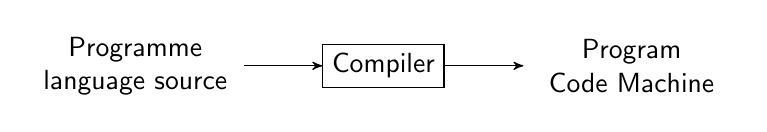
\begin{tikzpicture}
	\node[text width=2.5cm,align=center] (A) {Programme language source};
    \node[draw, shape=rectangle] (B) [right=of A] {Compiler};
	\node[text width=2.5cm,align=center] (C)[right=of B] {Program Code Machine};
	\path[->] (A) edge (B)
                (B) edge (C);
\end{tikzpicture}
\caption{Compilation}
\end{figure}


\subsubsection{Programming language}

\paragraph{Langage de programmation} Un langage artificiel dans lequel
un programmeur écrit un programme pour contrôler le comportement d'une
machine.


On définit un language de programmation en 3 étapes:
\begin{itemize}
    \item les \textbf{tokens}: "mot-clé" du langage
    \item la \textbf{syntaxe} et la \textbf{construction} du langage: comment écrire un programme qui fonctionne
    \item la \textbf{sémentique} du langage: sens des phrases.
\end{itemize}

\subsubsection{Machine language}

\paragraph{Langage machine (ou ensemble d'instructions)} est un langage
facilement interpreté par l'ordinateur lui-même. Chacune des
instruction occupe un byte ou plus et est facilement
acédé et interprété. On parle également d'architecture pour
l'ensemble d'instructions et le comportement d'une machine.

\paragraph{Complexité instruction}
On distringue plusieurs niveaux de complexités (CISC: \textit{Complex
Instruction Set Computer} ou RISC: \textit{Reduced Instructive Set Computer}).
Il faut plusieurs instructions RISC pour obtenir une instruction CISC.


Comme les registres sont très rapides, un ordinateur va essayer de
garder au maximum les données dans les registres.

\paragraph{Machine virtuelle} L'architecture est implémentée en software. Les étapes de l'analyse du compilateur pour produire le programme de sortie sont:
\begin{itemize}
	\item Mapper les noms aux adresses mémoires, frames de la pile et registres.
    \item Générer la liste linéaire des instructions machines.
    \item détecter les erreurs
\end{itemize}

\subsubsection{Interpreteur Vs Compilateur}

\begin{figure}[!h]
    \centering
    \begin{subfigure}[b]{0.4\textwidth}

        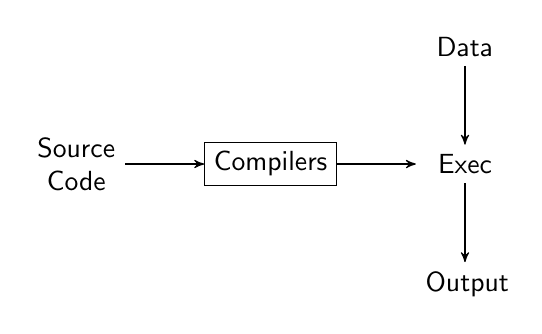
\begin{tikzpicture}
            \node[text width=1cm,align=center] (A) {Source Code};
            \node[draw, shape=rectangle] (B) [right=of A] {Compilers};
            \node[text width=1cm,align=center] (C)[right=of B] {Exec};
            \node[text width=1cm,align=center] (D)[above=of C] {Data};
            \node[text width=1cm,align=center] (E)[below=of C] {Output};


            \path[->] (A) edge (B)
            (B) edge (C)
            (D) edge (C)
            (C) edge (E);
        \end{tikzpicture}
    \end{subfigure}
    \quad
    \quad
    \begin{subfigure}[b]{0.4\textwidth}
        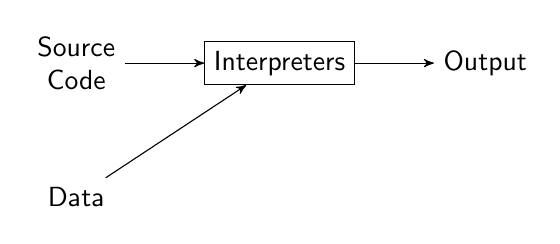
\begin{tikzpicture}
             \node[text width=1cm,align=center] (AA) {Source Code};
             \node[text width=1cm,align=center] (DD)[below=of AA] {Data};
             \node[draw, shape=rectangle] (BB) [right=of AA] {Interpreters};
             \node[text width=1cm,align=center] (EE)[right=of BB] {Output};

             \path[->] (AA) edge (BB)
             (DD) edge (BB)
             (BB) edge (EE);
         \end{tikzpicture}
     \end{subfigure}
     \caption{Compilation}
 \end{figure}

Dans le cas d'un interpréteur, le code high-level est exécuté directement.

 \paragraph{Avantages compilateur}:
\begin{itemize}
    \item \textbf{Performances}: le code machine est plus rapidement
exécuter, l'interpréteur doit lui redécoder à chaque fois les lignes
de codes pour les transformer en instructions.
    \item \textbf{Secret}: le code source est très difficile à déduire depuis un code machine.
\end{itemize}
\paragraph{Avantages interpréteur}:
\begin{itemize}
    \item L'overhead de l'interpreteur ne nécessite pas toujours la mise
        en place d'un compilateur (ex: les scripts)
    \item \textbf{Contrôle}: le code source est disponible, facilement modifiable.
    \item \textbf{Portabilité}: le langage machine dépend de la machine alors qu'un interpréteur est portable.
\end{itemize}

\subsection{Why should we study compilers?}
\begin{itemize}
	\item Ce sont de très grands programmes (comme ceux que nous étudirons plus tard)
    \item Il fait usage de tout ce que nous avons vu avant
    \item Cela permet d'apprendre sur le langage
    \item on en apprend sur la machine visée
    \item Il existe encore du boulot de compilation pour les nouveaux langages
    \item Ils se retrouvent partout
    \item Les programmes utilisent du XML se servent de technologies de compilation
    \item Mix de théorie et pratique
    \item Comme un compilateur peut être écrit en étapes, c'est un cas d'étude d'ingénérie logicielle
    \item écrire des programmes est chouette
\end{itemize}

\subsection{How does a compiler work? Phases of compilation}
On peut diviser en plusieurs étapes.

\begin{figure}[!h]
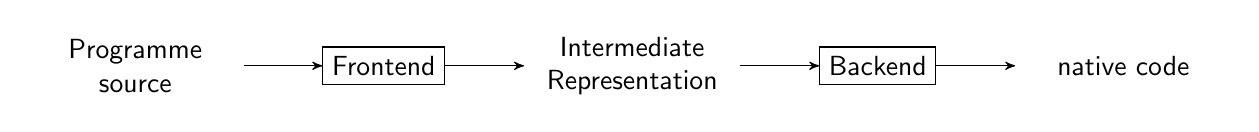
\begin{tikzpicture}
	\node[text width=2.5cm,align=center] (A) {Programme source};
    \node[draw, shape=rectangle] (B) [right=of A] {Frontend};
	\node[text width=2.5cm,align=center] (C)[right=of B] {Intermediate Representation};
    \node[draw, shape=rectangle] (D) [right=of C] {Backend};
	\node[text width=2.5cm,align=center] (E) [right=of D] {native code};
	\path[->] (A) edge (B)
              (B) edge (C)
              (C) edge (D)
              (D) edge (E);
\end{tikzpicture}
\caption{Compiler work}
\end{figure}

\subsubsection{Frontend}
\begin{itemize}
	\item Analyse du programme pour en deviner le sens
    \item dépend uniquement du langage de départ
    \item peut être décomposé:
\end{itemize}
\begin{figure}[!h]
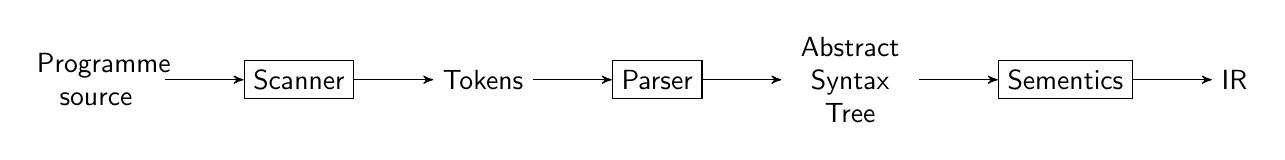
\begin{tikzpicture}
	\node[text width=1.5cm,align=center] (A) {Programme source};
    \node[draw, shape=rectangle] (B) [right=of A] {Scanner};
	\node (C)[right=of B] {Tokens};
    \node[draw, shape=rectangle] (D) [right=of C] {Parser};
	\node[text width=1.5cm,align=center] (E) [right=of D] {Abstract Syntax Tree};
    \node[draw, shape=rectangle] (F) [right=of E] {Sementics};
	\node (G) [right=of F] {IR};
	\path[->] (A) edge (B)
              (B) edge (C)
              (C) edge (D)
              (D) edge (E)
              (E) edge (F)
              (F) edge (G);
\end{tikzpicture}
\caption{Frontend}
\end{figure}

\subsubsection{Backend}
\begin{itemize}
	\item Prend le IR et produit le code machine
    \item Dépend de la machine d'arrivée uniquement
    \item peut-être décomposé en phases
\end{itemize}
\begin{figure}[!h]
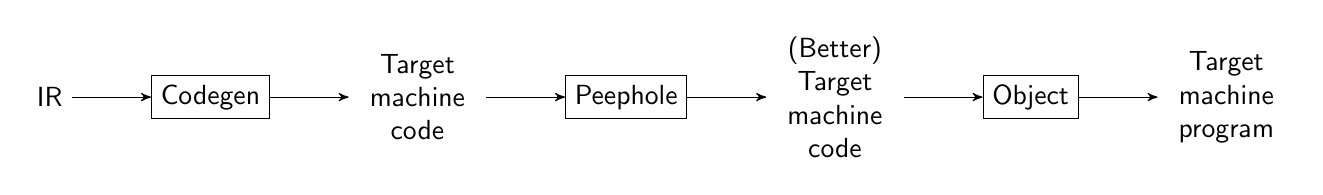
\begin{tikzpicture}
	\node (A) {IR};
    \node[draw, shape=rectangle] (B) [right=of A] {Codegen};
	\node[text width=1.5cm,align=center] (C)[right=of B] {Target machine code};
    \node[draw, shape=rectangle] (D) [right=of C] {Peephole};
	\node[text width=1.5cm,align=center] (E) [right=of D] {(Better) Target machine code};
    \node[draw, shape=rectangle] (F) [right=of E] {Object};
	\node[text width=1.5cm,align=center] (G) [right=of F] {Target machine program};
	\path[->] (A) edge (B)
              (B) edge (C)
              (C) edge (D)
              (D) edge (E)
              (E) edge (F)
              (F) edge (G);
\end{tikzpicture}
\captionsetup{singlelinecheck=off}
\caption[legend]{Backend :
    \centering
\begin{itemize}
	\item Codegen: Choisi les instructions adéquates
    \item Peephole: Cherche à faire un peu d'optimisation locale du code
    \item Object: liste les différents modules et construit un programme exécutable
\end{itemize}
}
\end{figure}

\subsubsection{Middle end}
Il peut y avoir l'ajout d'un optimisateur entre le frontend et le backend. Celui-ci à pour but d'améliorer le code intermédiare:
\begin{itemize}
	\item Il organise le programme en blocks
    \item Recherche la durée de vie des variables (next-use information)
    \item Élimine des sous-expressions et des \textit{constaints folding} ($x+4=9$ si on sait que $x=5$), regarde à l'allocation des registres
    \item Met les invariants hors des boucles, remplace les multiplication par des additions (car moins couteuse)
\end{itemize}

\subsubsection{Avantage de la décomposition}
\begin{itemize}
	\item Réduit la complexité
    \item Permet un dévelopement en parallèle
    \item Permet une réutilisation (un seul backend pour tous les langages pour une même machine)
\end{itemize}

\begin{figure}[!h]
    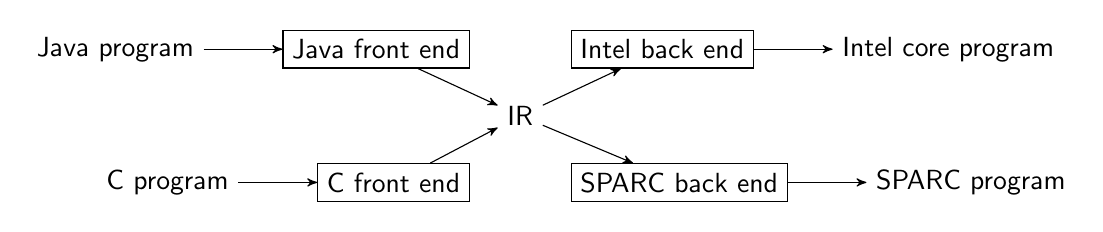
\begin{tikzpicture}
        \node (A1) {Java program};
        \node[draw, shape=rectangle] (B1) [right=of A1] {Java front end};

        \node (C) [below right=0.5cm of B1] {IR};

        \node[draw, shape=rectangle] (B2) [below left = 0.5cm of C] {C front end};
        \node (A2) [left = of B2] {C program};

        \node[draw, shape=rectangle] (C1) [above right =0.5cm of C] {Intel back end};
        \node (D1) [right = of C1] {Intel core program};

        \node[draw, shape=rectangle] (C2) [below right =0.5cm of C] {SPARC back end};
        \node (D2) [right = of C2] {SPARC program};

        \path[->] (A1) edge (B1)
        (A2) edge (B2)
        (B1) edge (C)
        (B2) edge (C)
        (C) edge (C1)
        (C) edge (C2)
        (C1) edge (D1)
        (C2) edge (D2);

    \end{tikzpicture}
    \caption{Decomposition}
\end{figure}


\subsubsection{Compiling to a Virtual Machine: New Boundaries}

\paragraph{.class}
Les programmes Java sont d'abord compilés en un fichier \texttt{.class}
(a \textbf{byte-code})
éxécutable sur la machine virtuelle. Le \texttt{.class} peut donc être
considérer comme un \textbf{IR} (Intermediate Representation), le
\texttt{JavaC} comme le frontend et la machine virtuel comme le
backend.

\paragraph{Machine virtuel}
La machine virtuelle est un interpréteur qui observe le code qu'on lui donne et
compile les parties critiques (\textit{hotspot}) qui sont les plus souvent
appelées. Il fait aussi du \textit{in-lining}, c'est-à-dire remplacer
des appels de méthode par leur code.

\paragraph{Note:}
Sur Windaube, ils ont implémenté une machine CLR (Commun Langage
Runtime). Suivant une technique appelée JIT (Just In Time), le CLR
compile chaque méthode en code natif et utilise ce code lorsque la
méthode est appelée.

\subsubsection{Compiling JVM code sur une architecture en registre}

En effet, le JVM code à une architecture basé sur la stack et il peut
y avoir différent challenge à résoudre pour mapper beacoup de variables 
vers un nombre limité de registre rapide.


La stratégie consistant à fournir du code intermédiare pour une
machine virtuelle a plusieurs avantages :

\begin{itemize}
	\item Le code intermédiare est compact
    \item De gros efforts ont eété fait pour optimiser ces machines virtuelles pour qu'elles s'exécute très rapidement (ex: Java, LOL)
    \item Le fait de ne compiler que les régions spéciales permettent d'aller plus vite que de compiler l'entièreté du code.
\end{itemize}

\subsection{An overview of the j-\-- to SVM compilers}

j-\-- est un sous-ensemble de Java: non-trivial, orienté objet,
supportant les classes, méthodes, champs, messages, statements,
expressions et types primitifs. 

Son compilateur est écrit en Java d'une manière orienté objet.

\subsubsection{j-\-- compiler organization}

Le début est la \texttt{main}. Après avoir lu les arguments, elle
crée le parser et le scanner. Ensuite:
\begin{itemize}
	\item \texttt{compilationUnit()} au parser pour obtenir l'AST.
    \item \texttt{preAnalyze()} au n\oe ud principal de l'arbre pour déclarer les types et classes dans la table des symboles.
    \item \texttt{analyze()} pour déclarer les noms et chercher les types
    \item \texttt{codegen()} pour gérer le code
    \item S'il y a des erreurs, on en cherche d'autres et puis on arrête.
\end{itemize}

\begin{figure}[!h]
    \includegraphics[width=\linewidth]{img/j--.png}
    \caption{j-\-- compiler}
\end{figure}

\subsubsection{Scanner}

Le scanner scanne les tokens à la demande et les classes en :
\begin{itemize}
    \item \textbf{Identifiant} (\texttt{main, myMethod})
    \item \textbf{tokens réservés} (\texttt{import, public, class, operateurs,
        separateurs,\ldots}) 
    \item \textbf{litéral} (tout le reste sans les séparateurs: \texttt{"Hello World", 3}, etc.).
\end{itemize}

\subsubsection{Parser}

Le parser est spécifique à la syntaxe du langage et est effectué en
\textit{recursive descent}.

\subsubsection{AST}

L'abstract syntax tree est une représentation sous forme d'arbre
du programme source. Il permet de rendre explicite la structure
syntaxique. Chacune des classes des nœuds étendent une même classe (\texttt{JAST})
et implémente 3 méthodes: 
\begin{itemize}
    \item \texttt{preAnalyze()} (déclarer les types) 
    \item \texttt{analyze()} (déclarer les variables locales) 
    \item \texttt{codegen()} (pour générer le code).
\end{itemize}

\subsubsection{Types}

Un type indique comment une varaible doit être interpreté et
se comporte. Java est dit statiquement typé car les types sont
déterminés à la compilation.


Dans le compilateur j-\--, on crée une classe type pour placer les
différents types.

%TODO

\subsubsection{Symbol table}

%TODO

\subsubsection{\texttt{preAnalyze()} and \texttt{analyze()}}

\paragraph{\texttt{preAnalyze()}} est le premier passage où l'on
vérifie le type. Il construit une partie de la table des symbol qui est
au dessus du AST (déclare les types importés et ceux déclarés par
les classes).

Ce passage est nécessaire pour déclaré les noms qui peuvent être référencé avant
leur définition.

\paragraph{\texttt{analyze()}} reprend là où \texttt{preAnalyze()} s'est arrêté.
Il s'occupe de:
\begin{itemize}
	\item Type checking: trouver le type de chaque expression
    \item Accessibilité: Regarde aux \texttt{public}, \texttt{protected} et \texttt{private}
    \item Member finding: vérifie les signatures.
    \item Tree rewriting: réécrit certains tree
\end{itemize}

\subsubsection{Stack Frames}

L'analise s'occupe aussi de calculer l'offset des variables locales
dans la stack frame (block continu de mémoire au-dessus de la pile
\textit{run-time}). On peut ainsi savoir l'espace repris par une
méthode à chacune de ses invocations.

\subsubsection{\texttt{codegen()}}

Permet de générer le byte code pour la JVM. Un outil
(\texttt{CLEmitter}) existe et permet de construire la table des
constantes et de générer les références utilisées par la JVM
pour les noms et constantes. Permet de calculer des offsets de
\textit{brckets} et les adresses. Calcule les coûts (espace mémoire)
des variables et l'espace de calcul nécessaire dans une méthode. Et
pour finir, il construit le fichier \texttt{.class}.

\subsubsection{j-\-- compiler source tree}

Pour ajouter une opération, on doit modifier le scanner pour
reconnaitre les nouveaux tokens, modifier le parser pour reconnaitre
l'expression, implémenter l'analyse sémentique et finalement la
génération du code allant avec cette opération.



\section{Chapitre 2 : Lexical Analysis} 
\subsection{Introduction}

\begin{figure}[!h]
    \centering
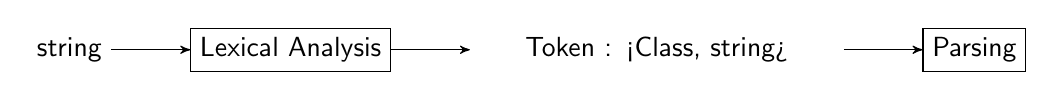
\begin{tikzpicture}
	\node (A) {string};
    \node[draw, shape=rectangle] (B) [right=of A] {Lexical Analysis};
	\node[text width=4.5cm,align=center] (C)[right=of B] {Token : <Class, string>};
    \node[draw, shape=rectangle] (D) [right=of C] {Parsing};
	\path[->] (A) edge (B)
              (B) edge (C)
              (C) edge (D);
\end{tikzpicture}

    \caption{Lexical analysis}
\end{figure}

L'analyse lexical parse donc l'input en une série de \textbf{token}.

\paragraph{Lexical tokens}: éléments composant les programmes. Ils
sont décrits par la syntaxe lexicale du langage.

\paragraph{Lexical analysis}: procédé permettant d'identifier
les lexical tokens dans le programme. On peut séparer les tokens
lexicaux en catégories: 
\begin{itemize}
    \item les identifiants
    \item les mots réservés, opérateurs et séparateurs
    \item les literaux
\end{itemize}

\subsection{Scanning tokens}

\paragraph{Scanner} Un scanner est un programme
écrit par le programmeur (\textit{handwritten}) ou bien générée
automatiquement par une liste de regex . 

Les espaces peuvent servir à séparer des tokens mais pas tout le temps, par 
exemple si on est entrain de scanner un \texttt{integer} et que l'on tombe
sur une lettre, on peut en conclure que l'\texttt{integer} est fini.

\subsection{Lexical analysis hand written}

Dans le cas d'un scanner écrit à la main, il est très utile de
décrire le scanner comme un \textbf{state transition diagram}.

\subsubsection{State transition diagram} diagramme dans lequel les nœuds
représentent les états, les flèches dirigées représentes des
mouvement d'un état à l'autre suivant ce qui est scanné. Si un
caractère scanné n'est sur aucune flèche, on choisi celle non
étiquetée.

\paragraph{Implémentation}

\begin{itemize}
    \item Les choix sont représenté par des \texttt{if} (ou \texttt{switch})
    \item Les cyles sont des \texttt{while}
    \item Les mots réservés ne sont pas intégré dans la machine à
        états car cela est trop complexe. A la place on liste les 
        mots réservés dans une table et faire un \textit{lookup} à chaque
        fois qu'on reconnait un identifiant. 
    \item Les opérateur sont intégré dans la machine à états finis (via un
        \texttt{switch} entre les différents opérateurs possible)
    \item Les espaces sont ignorés (indique la fin d'un token)
    \item Les commentaires sont ignorés
\end{itemize}


\subsection{Lexical analysis generator}
\subsubsection{Regular Expressions (regex)}

On dit que les regex définissent un langage de strings sur un alphabet.

Les regex peuvent prendre les formes suivantes:
\begin{itemize}
    \item Si $a$ est dans l'alphabet, alors le regex a décrit le langage
        consistant en les strings $a$. On appelle ce langage $L(a)$

    \item Si $r$ et $s$ sont des regex, alors leur concaténation $rs$
        est aussi une regex décrivant le langage de tous les strings possibles
        obtenus par concaténation d'un string du langage $r$ et d'un string de
        langage $s$. On appelle ce langage $L(rs)$

    \item Si $r$ et $s$ sont des regex, $L(r|s)$ décrit le langage
        composé des strings de l'un ou l'autre langage

    \item Si $r$ est un regex, $L(r*)$ décrit le langage formé par
        concaténation de zéro ou plusieurs instances de $r$ ($\epsilon$
        représente la string vide)

    \item $\epsilon$ est le langage contenant uniquement la string vide

    \item $r$ et $(r)$ sont les mémes regex. Les parenthèses sont
        utilisées pour grouper les regex.

\end{itemize}

\subsubsection{Finite State Automate (FSA)}

Pour tout langage décrit par une regex, il existe un diagramme à
transition d'état. 

\textit{Un automate fini reconnait un language.}

\paragraph{Automate à états finis} (Finite State Automate) c'est $F =
(\Sigma, S, s_0, M, F)$ où:

\begin{itemize}
	\item $\Sigma$ est l'alphabet
    \item $S$ est l'ensemble des états
    \item $s_0 \in S$ est l'état initial
    \item $M$ est l'ensemble de mouvements possibles d'un état à un
        autre ; $M(r, a) = S$ où $r, s \in S$ et $a \in \Sigma$
    \item $F \in S$ est l'ensemble des états finaux
\end{itemize}

\paragraph{Une phrase appartient au language} si en partant du start, on
arrive sur un état final après avoir suivit les changement d'états
correspondant à la phrase.

Il existe un moyen automatique de générer un FSA à partir de regex.

\subsubsection{Non-Deterministic Finite State Automate (NFA) vs. Deterministic FSA (DFA)}

\paragraph{\textbf{DFA}} automate à états finis où il n'y a pas de
$\epsilon$-move et où un seul chemin existe à partir d'un état pour
un input.

On ne peut donc aps avoir $M(r, a) = s$ et $M(r, a) = t$ tel que $s \neq t$.

\begin{itemize}
    \item DFA are faster to execute and easy to implement (by
        table driven implementation)
\end{itemize}

\paragraph{\textbf{NFA}} automate à états finis qui permet plusieurs chemins
à partir d'un état pour le même input, et autorise $\epsilon$-move.

\begin{itemize}
    \item NFA are in general smaller (exponentially)
\end{itemize}

\subsubsection{Regular expressions to NFA}

On utilise les constructions de \textbf{Thompson}:
\begin{itemize}
	\item $a$:\\
    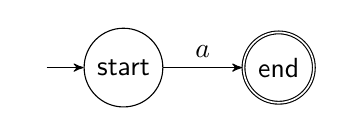
\begin{tikzpicture}
		\node[state] (A) [initial, initial text={}] {start};
    	\node[state] (B) [right=of A, accepting] {end};
		\path[->] (A) edge node[above] {$a$} (B); % [bend left]
	\end{tikzpicture}
	\item $rs$:\\
    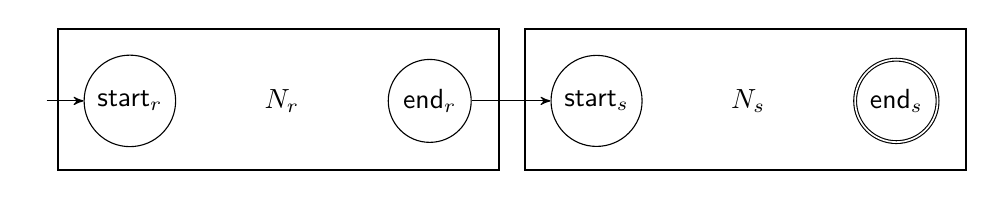
\begin{tikzpicture}
		\node[state] (A) [initial, initial text={}] {start$_r$};
    	\node        (B) [right=of A] {$N_r$};
    	\node[state] (C) [right=of B] {end$_r$};
		\node[state] (D) [right=of C] {start$_s$};
    	\node        (E) [right=of D] {$N_s$};
    	\node[state] (F) [right=of E, accepting] {end$_s$};
		\path[->] (C) edge (D);
        \draw[thick] ($(A.north west)+(-0.5,0.5)$) rectangle ($(C.south east)+(0.5,-0.5)$);
        \draw[thick] ($(D.north west)+(-0.5,0.5)$) rectangle ($(F.south east)+(0.5,-0.5)$);
	\end{tikzpicture}
	\item $r|s$:\\
    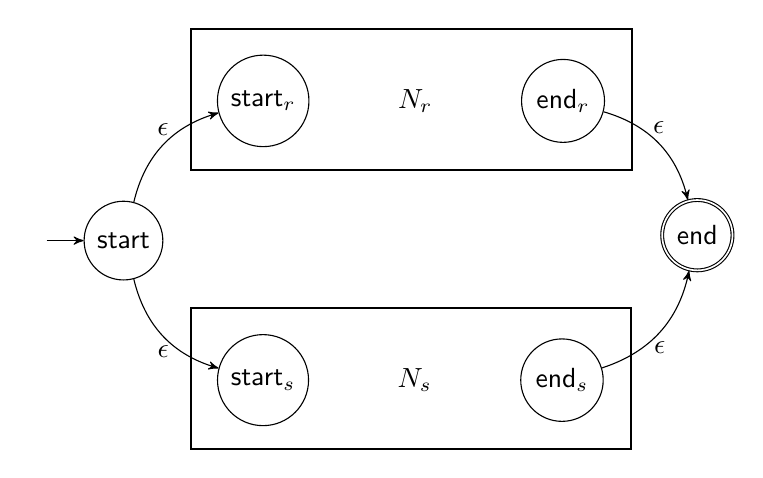
\begin{tikzpicture}
    	\node[state] (0) [initial, initial text={}] {start};
		\node[state] (A) [above right=of 0]{start$_r$};
    	\node        (B) [right=of A] {$N_r$};
    	\node[state] (C) [right=of B] {end$_r$};
		\node[state] (D) [below right=of 0] {start$_s$};
    	\node        (E) [right=of D] {$N_s$};
    	\node[state] (F) [right=of E] {end$_s$};
    	\node[state] (G) [below right=of C, accepting]{end};
		\path[->] (0) edge[bend left] node[above] {$\epsilon$} (A);
		\path[->] (0) edge[bend right] node[below] {$\epsilon$} (D);
		\path[->] (C) edge[bend left] node[above] {$\epsilon$} (G);
		\path[->] (F) edge[bend right] node[below] {$\epsilon$} (G);
        \draw[thick] ($(A.north west)+(-0.5,0.5)$) rectangle ($(C.south east)+(0.5,-0.5)$);
        \draw[thick] ($(D.north west)+(-0.5,0.5)$) rectangle ($(F.south east)+(0.5,-0.5)$);
	\end{tikzpicture}
	\item $r*$:\\
    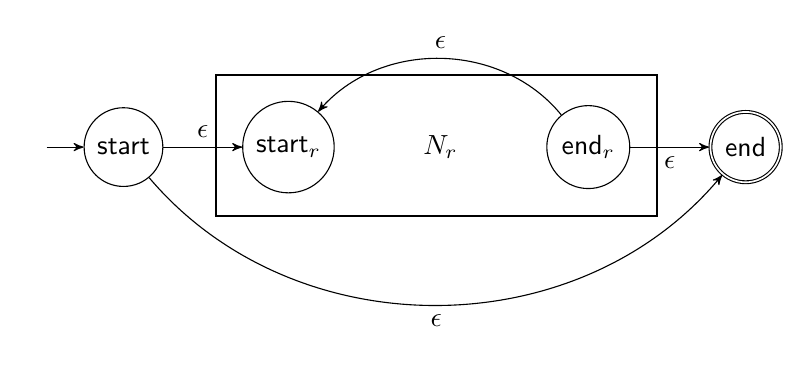
\begin{tikzpicture}
    	\node[state] (0) [initial, initial text={}] {start};
		\node[state] (A) [right=of 0]{start$_r$};
    	\node        (B) [right=of A] {$N_r$};
    	\node[state] (C) [right=of B] {end$_r$};
    	\node[state] (D) [right=of C, accepting]{end};
		\path[->] (0) edge node[above] {$\epsilon$} (A);
		\path[->] (0) edge[bend right=50] node[below] {$\epsilon$} (D);
		\path[->] (C) edge[bend right=50] node[above] {$\epsilon$} (A);
		\path[->] (C) edge node[below] {$\epsilon$} (D);
        \draw[thick] ($(A.north west)+(-0.5,0.5)$) rectangle ($(C.south east)+(0.5,-0.5)$);
	\end{tikzpicture}
	\item $\epsilon$:\\
    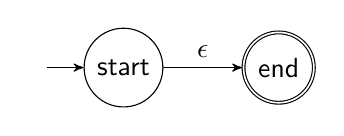
\begin{tikzpicture}
		\node[state] (A) [initial, initial text={}] {start};
    	\node[state] (B) [right=of A, accepting] {end};
		\path[->] (A) edge node[above] {$\epsilon$} (B);
	\end{tikzpicture}
\end{itemize}

\subsubsection{NFA to DFA}

Il est évident qu'un NFA nécessite du \textbf{backtracking} poour
parser un input (puisqu'il peut emprunter le mauvais choix) qui prend du
temps\ldots Heureusment, pour toutes NFA il existe une DFA équivalente.
On arrive à la trouver grâce aux $\epsilon$-closure.


\paragraph{$\epsilon$-closure($s$)} c'est un ensemble incluant $s$ ainsi
que tous les états atteignables à partir de $s$ uniquement avec
des $\epsilon$-moves.

\paragraph{$\epsilon$-closure($S$)} c'est un ensemble incluant
l'ensemble $S$ ainsi que tous les états atteignables à partir de
chaque élément $s$ de $S$ uniquement avec des $\epsilon$-moves.

\begin{figure}
\begin{lstlisting}[mathescape]
Input: a set of states, S.
Output: $\epsilon$-closure(S)

Stack P.addAll(S);     
Set C.addAll(S);       
while (!P .empty() ) {
    s = P.pop();
    for (r $\in$  move(s, $\epsilon$)){
        if (r $\notin$ C) {
            P.push( r );
            C.add( r );
        }
    }
}
return C;
\end{lstlisting}
\caption{$\epsilon$-closure algorithm}
\end{figure}

\begin{figure}
\begin{lstlisting}[mathescape]
Input: an NFA, N = ($\sum$, S, $s_0$ , M, F)
Output: DFA, D = ($\sum$, $S_D$ , $s_{D0}$ , $M_D$ , $F_D$ )

Set $S_{D0}$ = $\epsilon$-closure($s_0$ );
Set $S_D$ .add($S_D0$ );
Moves $M_D$ ;
Stack stk.push($S_{D0}$ );
i = 0;
while (! stk.empty()) {
    t = stk.pop();
    for (a : $\sum$) {
        $S_{Di+1}$ = $\epsilon$-closure(M(t, a));
        if ($S_{Di+1}$ != {}) {
            if ($S_{Di+1}$ $\notin$ $S_D$ ) {
                // We have a new state.
                $S_D$ .add($S_{Di+1}$ );
                stk.push($S_{Di+1}$ );
                i = i+ 1;
                $M_D$ .add($M_D$(t, a) = i ) ;
            }
            else if ($\exists$ j, $S_j \in S_D$ $\wedge$ $S_{Di+1} == S_j$ ) {
                .. In the case that the state already exists.
                $M_D$ .add($M_D$(t,a) = j ) ;
            }
        }
    }
}

Set $F_D$ ;
for ($s_D$ : $S_D$ )
    for (s : $s_D$ )
        if (s $\in$ F)
            $F_D$ .add($s_D$ );

return D = ($\sum$, $S_D$ , $s_{D0}$ , $M_D$ , $F_D$ );

\end{lstlisting}
\caption{DFA construction algorithm}
\end{figure}

%TODO : explication algorithm

\subsubsection{Minimal DFA}

L'idée est de fusionner des états non-distinguable (càd qu'on ne peut
distinguer d'un autre pour chaque input). On va recréer des états
grace à des partitions.

\paragraph{Partitions}
\begin{itemize}
    \item Les partitions initialles sont \textit{final} et \textit{non-final}. 
    \item On scinde en différente partition quand les états sont distinguables
    \item Pour chaque partition, un input doit induire un mouvement vers
        une même partition.

    \item[Note:] On doit s'assurer que pour chacun des états, le mouvement d'un symbole
        particulier reflète celui dans l'ancien DFA. 
\end{itemize}

\subsubsection{Table driven}

For each DFA, a Table driven can be implemented as a 2D table (states
and input).

For every $M(r, a) = s$, $T[r, a] = s$.

\paragraph{Recognize the longest match}

Un automate reconnait les états finaux avec deux variables :
\begin{itemize}
    \item \texttt{Last-Final} : le dernier état final rencontré
    \item \texttt{Input-Position-at-Last-Final}
\end{itemize}

On met à jour ces deux variables quand un état final est rencontré.
Quand a \textit{dead} état (càd un état qui n'a pas l'ouput correspondant
à l'input) est atteint, les variables disent quels tokens ont matché et où ils
se sont fini.

\subsubsection{JavaCC: Tool for generating scanner}

JavaCC est un outil pour générer une analyse lexicale à partir de
regex ainsi qu'un parseur à partir d'une grammaire hors contexte.


Lorsque l'on scanne un token, on considère tous les regex correspondant
à l'état actuel et on choisi celui qui contient le plus de
caractères.


Il existe 4 types de regex:
\begin{itemize}
	\item SKIP: regex jeté
    \item MORE: on continue après
    \item TOKEN: crée un token et est retourné au parseur
    \item SPECIAL-TOKEN: crée un token spécial ne participant pas au parsing
\end{itemize}

\section{Chapitre 3 : Parsing}

\subsection{Introduction}

\paragraph{Parsing} action de mettre les tokens ensemble pour créer des
entités syntaxiques plus grandes (expressions, instructions, méthodes,
définition de class, ...).

Fonction du parsing :
\begin{itemize}
    \item Assumer la validité syntaxique du programme. 
        \begin{enumerate}
            \item Identifier une erreur et la reporter
                (erreur et le numéro de ligne). 
            \item Ne pas s'arrêter après une erreur et chercher d'autres erreurs
                (pour ne pas reporter qu'une seule erreur à la fois). 
        \end{enumerate}
    \item Fournir une représentation du programme parsé, souvent en
    arbre (\textbf{AST}) car ce type de représentation est facile à
    analyser et à "décorer" d'informations.

\end{itemize}

\subsection{Context-Free Grammars and Languages}

CFG est plus puissant que RegExp. En effet, impossible en RegExp
de décrire un string tel que une suite de ``a'' est suivit d'une suite de ``b''
tel que les deux séquences ont la même taille.

Cela est impossible puisque les DFA ne peuvent pas compter!

\subsubsection{Backus-Naur Form (BNF) and its extensions}

On définit les langages de programmation de manière récursive.
\begin{itemize}
	\item[$::=$] : "\textit{peut être écrit comme}", sigle de la définition
    \item[$|$] : "ou"
    \item[$[X\rfloor$] : $X$ est optionnel
    \item[$\{X\}$] : \textit{Keene closure}, $X$ apparait de 0 à plusieurs fois.

\end{itemize}

\subsubsection{Grammar and the Language it describes}
\paragraph{Context-Free grammar} Une grammaire sans contexte est un tuple $G=(N,T,S,P)$ où:
\begin{itemize}
	\item[$N$] est un ensemble de symboles non terminaux
    \item[$T$] est un ensemble de symboles terminaux
    \item[$S \in N$] est un non terminal appelé symbole de départ
    \item[$P$] est un ensemble de règles de production
\end{itemize}

\paragraph{Derivation} Séquence d'applications de règles de
production, démarrant du symbole de départ pour arriver à
l'expression voulue («~$\Rightarrow$~» est le symbole de la relation
de dérivation).

\paragraph{Directly derive} Lorsqu'un string de symboles dérive d'un
autre en une seule étape.

\subparagraph{E directly derives T + T} :
$ E \Rightarrow T + T$

\paragraph{Language $L(G)$} On dit que le langage $L(G)$, décrit par
une grammaire $G$, consiste en tous les strings ne comprenant que des
symboles terminaux pouvant être dérivés du symbole de départ.

\paragraph{Left-most derivation} Dérivation dans laquelle, à chaque
étape, le string suivant est dérivé en applicant une règle de
production réécrivant le non terminal le plus à gauche.

\paragraph{Right-most derivation} Dérivation dans laquelle, à chaque
étape, le string suivant est dérivé en applicant une règle de
production réécrivant le non terminal le plus à droite.

\paragraph{Sentential form} Chaque string de terminaux ou non terminaux
qui peut être dérivé à partir d'un symbole de départ.

\paragraph{Parse tree} Arbre illustrant les dérivations effectuées
depuis un symbole de départ (racine) pour arriver à une expression
(feuilles).

\subsubsection{Ambiguous Grammars and unambiguous grammars}

Detecter si une context free grammar est ambiguous est \textbf{indécidable}.
Notons que les grammaires LL(k) et LR(k) sont non-ambiguous.

\begin{itemize}
    \item \textbf{Ambiguous sentence} : Une phrase par laquelle il existe
        plusieurs dérivations possibles. (2 arbres pour représenter $id + id * id$)
\item \textbf{Ambiguous grammar} : Une grammaire qui décrit au-moins une
        phrase ambigüe.
    \item \textbf{Unambiguous grammar} : Une grammaire ne décrivant que
        des phrases à dérivation unique (qu'elle soit \textit{left} ou
        \textit{right}). 
\end{itemize}

\paragraph{IF..ELSE ambiguous}
Pour résoudre cet ambiguité, on définit une règle telle que
le \texttt{else} se groupe avec le \texttt{if} précédent.

\begin{center}
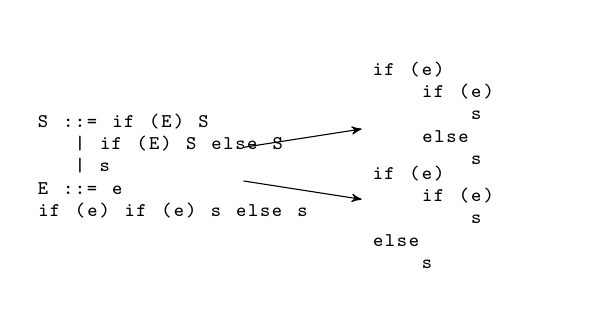
\begin{tikzpicture}
    \node[text width=2.5cm,align=center] (A) 
    {{\begin{lstlisting}[basicstyle=\ttfamily\scriptsize]
S ::= if (E) S
   | if (E) S else S
   | s
E ::= e
if (e) if (e) s else s
\end{lstlisting}}};

	\node[text width=2.5cm,align=center,  above right=-1.5cm and 1.5cm of A] (B) 
	{{\begin{lstlisting}[basicstyle=\ttfamily\scriptsize]
if (e)
    if (e)
        s
    else
        s
\end{lstlisting}}};
	\node[text width=2.5cm,align=center, below right=-1.5cm and 1.5cm of A] (C) 
	{{\begin{lstlisting}[basicstyle=\ttfamily\scriptsize]
if (e)
    if (e)
        s
else
    s
\end{lstlisting}}};

		\path[->] (A) edge (B)
		(A) edge (C);

\end{tikzpicture}
\end{center}


\paragraph{x.y.z ambiguous}

Il y a aussi ambiguité avec $x.y.z$: est-ce un \textit{field
selection}, un nom de package, un nom de class, etc. 


Pour résoudre cela, un nœud \texttt{Ambiguous Name} est placé dans
l'\textbf{AST} et est revu par le compileur après la déclation des types
(\textit{type declaration}).


\subsubsection{Parseur}

Pour les parseur des langages décrits par une grammaire
\textit{context-free}, on utilise une \textit{pushdown} stack avec
\textit{backtracking}.

Lorsque le \textit{backtracking} n'est pas nécessaire, on parle de
parsing déterministe. Deux types de parsing déterministes:

\begin{itemize}
    \item Top-Down: le parser commence avec le \texttt{start symbol}
        et étape par étape dérive l'input sentence pour produire l'\textbf{AST}
        du root aux feuilles.
    \item Bottom-up: le parser commence avec l'input sentence et le scanne
        de gauche à droite et applique les règles. L'\textbf{AST} est construit
        du bas vers le root.
\end{itemize}


\subsection{Top-Down Deterministing Parsing}

Deux types de top-down: 
\begin{itemize}
    \item recursive descent 
    \item $LL(1)$. 
\end{itemize}

Le parser commence au symbol de départ (root) et agrandit 
l'AST en déscendant vers les feuilles\ldots il remplace le symbole
par le coté droite d'une règle BNF.

Il va scanner la phrase d'input et parser les entités syntaxique
représentées par le symbole de départ.

\subsubsection{Parsing by recursive descent}

Parser par descente récursive invoque une procédure écrite
pour parser chaque non-terminal selon qui lui est associé.
La procédure choisit la règle a appliquer selon le prochain non-scanné
symbol. (Ne nécessite pas de backtracking!)

Ces méthodes construisent également les nœuds AST!

\paragraph{Utils}
Le scanner a quelques méthodes utiles pour aider à décider de la
règle de production adéquate :

\begin{itemize}
    \item \texttt{have(TOKEN)}: renvoie \texttt{true} si le token est présent, 
        et le scanne.
    \item \texttt{mustBe(TOKEN)}: renvoie \texttt{true} si le token est
        présent et le scanne ou une erreur sinon.
    \item \texttt{see(TOKEN)}: regarde si le token est présent dans le scanner.
\end{itemize}

\paragraph{Lookahead}
%TODO
Pour certaines grammaires, il faut regarder plus loin que le token
suivant pour savoir ce qui est présent en premier et pour savoir
quelle loi de dérivation utiliser. On a un \textit{Lookahead} scanner
définit qui permet de voir plus loin qu'un symbole. 

\paragraph{Error recovery}
%TODO 
Pour récupérer des erreurs, les \texttt{mustBe}, lorsqu'il rencontre
un token inatendu, scanne jusqu'à trouver celui qu'il veut jusqu'à se
remettre dans un état à nouveau correct.

\subsubsection{$LL(1)$ parsing}

Contrairement au recursive descent, ici, la stack est explicite.
Le 1\ier $L$ veut dire \textit{left-to-right scan}, le 2\ieme pour
\textit{left-most derivative} et le $1$ pour le fait qu'on regarde un
seul symbole à la fois.\\


Chaque grammaire a une table de parsing unique. Pour créer la table, si
$\alpha$ et $\beta$ sont des strings (pouvant être vides) de terminaux
et non terminaux : 
\begin{center}
$table[Y,a]=i$ où $i$ est le numéro de la règle,
$Y ::= X_1, X_2,..., X_n$ si soit $X_1, X_2,..., X_n \Rightarrow
a\alpha$ ou $X_1, X_2,..., X_n \xrightarrow{*} \epsilon$ et il y a une
dérivation $S$\# $ \Rightarrow \alpha Y a \beta$.\\
\end{center}

Pour arriver à établir cette table, on fait usage de deux ensemble :
\texttt{first} et \texttt{follow}.


\paragraph{LL(1) parsing algorithm}

Au tout début, on place le symbole terminal initial sur la pile.
Suivant le token scanné, on remplace le symbole sur la pile par celui
qui correspond suivant la table de parsing. 

Lorsqu'un non-terminal est trouvé sur la pile et si c'est bien celui
qui est scanné, il est retiré de la pile et un nouveau token est
scanné.

\begin{lstlisting}
Initially,
Stack stk initially contains the terminator # and the start symbol S, with S on top;
Symbol sym points to the first symbol in the sentence w.
for (;;) {
    Symbol top = stk.pop();
    if (top == sym == #) halt successfully;
    else if (top is a terminal symbol) {
        if (top == sym) {
            advance sym to point to the next symbol in w;
        } else {
            halt with error: a sym found where a top was expected;
        }
    } else if (top is a non-terminal, Y) {
        int index = table[Y,sym];
        if (index != err)} {
        rule = rules[index];
        Say rule is Y ::= X 1 X 2 ...X n
        Push X n,..., X 2, X 1 onto the stack stk, with X 1 on top
        }
        else {
            halt with an error.
        }
    }
}

\end{lstlisting}

\paragraph{First}
%TODO : rendre joli

Correspond à l'ensemble des terminaux qui peuvent commencer une règle.
\textbf{First may contain $\epsilon$ ($X_1 X_2 ... X_n \Rightarrow *
\epsilon$)}

$$first(X_1 X_2 ... X_n) = \{ a \quad | \quad X_1 X_2 ... X_n
\Rightarrow * a \alpha, a \in T\}$$

\begin{enumerate}
    \item Calcul de $first(X)$ pour tous les $X$ dans la grammaire:
        \begin{lstlisting}[mathescape]
For each terminal $x$, $first(x) = \{x\}$.
For each non-terminal $X$, $first(X) = \{\}$.
If there is a rule $X ::= \epsilon$ in $P$, add $\epsilon$ to $first(X)$.

Repeat until no new symbols are added to any set: 
    For each rule$ Y ::= X_1 X_2 ... X_n \in P$ 
        add all symbols from $first(X_1 X_2 ... X_n)$ to $first(Y)$.
        \end{lstlisting}

    \item Calcul de $first(X_1 X_2 ... X_n)$:
        \begin{lstlisting}[mathescape]
Set S = first(X$_1$).
i = 2
While $\epsilon$ $\in$ S and i $\le$ n {
    S = S - $\epsilon$
    Add first(X$_i$) to S
    i = i+1
return S
\end{lstlisting}
\end{enumerate}

\paragraph{Follow}

Correspond à l'ensemble des terminaux qui peuvent suivre une règle.
\textbf{First cannot contain $\epsilon$ }

$$follow(X) = \{ a \quad | \quad S \Rightarrow * wX\alpha and \alpha \Rightarrow * a ...\}$$

Calcul de $follow(X)$:
\begin{lstlisting}[mathescape]
$follow(S) = \{$\#$\}$.
$follow(X) = \{\}$ for all non-terminals X $\ne$ S.
Repeat until no new symbols are added to any set:
    for each rule $Y ::= X_1 X_2... X_n \in P$,
        for each non-terminal $X_i$,
            add $first(X_{i+1} X_{i+2}... X_n) - {\epsilon}$ to $follow(X_i)$, and
            if $X_i$ is the rightmost symbol or $first(X_{i+1} X_{i+2}... X_n)$ contains $\epsilon$,
                 add $follow(Y)$ to $follow(X_i)$.

\end{lstlisting}

\paragraph{Parsing table}

Construire une table de parsing $LL(1)$ pour une grammaire $G=(N,T,S,P)$:\\
For each non-terminal $Y$ in $G$,\\
\hspace*{1em}For each rule $Y ::= X_1 X_2...X_n \in P$ with number $i$,\\
\hspace*{2em}For each terminal $a$ $\in$ $first(X_1 X_2... X_n) - \{\epsilon\}$, add $i$ to $table[Y, a]$.\\
\hspace*{2em}If $first(X_1 X_2... X_n)$ contains $\epsilon$, for each terminal (or \#) in $follow(Y)$, add $i$ to $table[Y, a]$.\\

Une grammaire est dite $LL(1)$ si la table de parsing produite n'a pas de conflits. Toute grammaire $LL(1)$ est non ambigue.\\
On peut avoir des grammaire non $LL(1)$ mais $LL(k)$ avec $k>1$ (on regarde alors $k$ symboles). On peut transformer certaines grammaires non $LL(1)$ en une équivalente $LL(1)$  dans certains cas:
\begin{align*}
	\text{left recursive: } X &::= X\alpha & X &::= \beta X'\\
    X &::= \beta & \Rightarrow X' &::= \alpha X'\\
    & & X' &::= \epsilon\\
    \text{left factoring: } X &::= \alpha \beta & X &::= \alpha X'\\
    X &::= \alpha \gamma & \Rightarrow X' &::= \beta\\
    & & X' &::= \gamma     
\end{align*}


\paragraph{Error recovery}
Si il reçoit un input non attendu pour terminal/non-terminal ($T$) dans la stack,
il va simplement skipper les tokens jusqu'a obtenir un token $\in$ Follow($T$).

\subsubsection{Left recursion removal}

\paragraph{Regle typique pour supprimer la left recursion}
\begin{center}
\begin{tikzpicture}
    \node[text width=2.5cm,align=center] (A) 
    {{\begin{lstlisting}
Y ::= Y a
Y ::= b
\end{lstlisting}}};

	\node[text width=2.5cm,align=center,  right= of A] (B) 
	{{\begin{lstlisting}[mathescape]
Y  ::= bY'
Y' ::= aY'
Y' ::= $\epsilon$
\end{lstlisting}}};
		\path[->] (A) edge (B);

\end{tikzpicture}
\end{center}

\paragraph{Indirect left recursion}
Dans ce cas la, une première manipulation est nécessaire avant
d'appliquer la régle de base.

\begin{center}
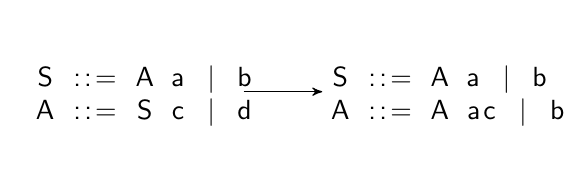
\begin{tikzpicture}
    \node[text width=2.5cm,align=center] (A) 
    {{\begin{lstlisting}
S ::= A a | b
A ::= S c | d
\end{lstlisting}}};

	\node[text width=2.5cm,align=center,  right= of A] (B) 
	{{\begin{lstlisting}
S ::= A a | b
A ::= A ac | bc | d
\end{lstlisting}}};
		\path[->] (A) edge (B);

\end{tikzpicture}
\end{center}


\subsection{Bottom-up deterministic parsing}
On passe!!

\subsection{Parser Generation using Java CC}

On utilise une structure syntaxique EBNF (\textit{extended BNF}). On
peut définir ainsi des parseurs $LL(k)$ récursive descent. Le fichier
\texttt{j--.jj} contient donc les regex pour la structure lexicale ainsi
que les règles syntaxiques du langage.


Entre \texttt{PARSER\_BEGIN(JavaCCParser)} et
\texttt{PARSER\_END(JavaCCParser)} sont définies des fonctions utiles
et utilisées dans le parser généré : \texttt{reportParserError()} et
\texttt{recoverFromError()}.


\subsubsection{Specification syntaxique}

La syntaxe EBNF est:
\begin{itemize}
	\item $[a]$: 0 ou 1
    \item $(a)^*$: 0 ou plusieurs
	\item $a|b$: $a$ ou $b$
    \item $()$: grouping
\end{itemize}

\subsubsection{Déclaration de symbol non-terminaux}

On définit premièrement un symbole de départ
(\texttt{compilationUnit}) qui est un ``haut niveau'' de non-terminal
et référence le niveau inférieur de non-terminal. Ceux ci reference
les tokens définit dans la spécification lexical.

La déclaration de non terminaux ressemble à une méthode java. Il y a
un type de retour, un nom, peut avoir des arguments et à un corps de
méthode. Il y a un bloc précédent celui-là dans lequel les variables
locales sont déclarées.

%TODO : example page 70 chapitre 03

\subsubsection{Lookahead}
Lorsqu'il est nécessaire de regarder plusieurs symboles après
l'actuel, on utilise la méthode \texttt{LOOKAHEAD(<token>)}. 

Il y a deux méthodes pour récupérer des erreurs : \textit{shallow}
et \textit{deep} (utilisé par j-\--). Dans le corps d'un non terminal,
on catch les erreurs du parseur. On choisit alors à quel token on veut
reprendre (\textit{skip to token}). Il y a donc premièrement affichage
d'une erreur puis récupération par shipping. 

\subsubsection{Avantage}
Les avantages d'un parser autogénéré (JavaCC) sont:

\begin{itemize}
	\item Structure lexicale mieux expliquée
    \item Construction EBNF possible
    \item Lookahead possible et facile
    \item Conflit de choix reporté
    \item Mécanisme de récupération d'erreur sophistiqué utilisable.
\end{itemize}


\subsection{Bactracking parsing (not in the book)} %LN

Avec le backtracking parsing, on peut parser n'importe quel langage
décrit par une CFG. On va dériver en left most à partir du symbol
initial en choisisant la première règle de dérivation. Tant que les
terminaux déjà obtenu match le string qu'on veut matcher alors on
continue, sinon on revient à l'étape pérédente et on choisit la
règle de dérivation suivante.

Exemple:

Suivant la grammaire :
\begin{lstlisting}
S ::= ASA
S ::= ASB
S ::= A
A ::= a
B ::= b
\end{lstlisting}

Si on souhaite parser $aab$, on a les étapes suivantes :
\begin{lstlisting}
S
S => ASA
S => ASA => aSA
S => ASA => aSA => aASAA
S => ASA => aSA => aASAA => aaSAA
S => ASA => aSA => aASAA => aaSAA => aaASAAA
S => ASA => aSA => aASAA => aaSAA => aaASAAA => aaaSAAA
!! backtrack !!
S => ASA => aSA => aASAA => aaSAA => aaASAAA
!! backtrack a nouveau car pas d autre regle pour A !!
S => ASA => aSA => aASAA => aaSAA
S => ASA => aSA => aASAA => aaSAA => aaASBAA
S => ASA => aSA => aASAA => aaSAA => aaASBAA => aaaSBAA
!! backtrack !!
S => ASA => aSA => aASAA => aaSAA => aaASBAA
!! backtrack a nouveau car pas d autre regle pour A !!
S => ASA => aSA => aASAA => aaSAA
S => ASA => aSA => aASAA => aaSAA => aaAAA
S => ASA => aSA => aASAA => aaSAA => aaAAA => aaaAA
!! backtrack !!
S => ASA => aSA => aASAA => aaSAA => aaAAA
!! backtrack a nouveau car pas d autre regle pour A !!
S => ASA => aSA => aASAA => aaSAA
!! backtrack a nouveau car pas d autre regle pour S !!
S => ASA => aSA => aASAA
!! backtrack a nouveau car pas d autre regle pour A !!
S => ASA => aSA
S => ASA => aSA => aASBA
S => ASA => aSA => aASBA => aaSBA
... (on a compris l idee)
\end{lstlisting}

\subsection{Packrat parsing (not in the book)} %LN

Pour éviter le coût du backtrack parsing (qui peut être exponentiel
si à chaque fois on se retrouve à devoir prendre la dernière
dérivation), on utilise de la mémorization. On obtient donc un
algorithme en O(input*\#production).

On va pour chaque index dans l'input essayer de parser via toutes les
règles possibles et stocker le résultat ainsi que l'index de fin de
l'expression. On peut ainsi aller de l'index le plus grand au plus petit
en utilisant les résultats précedemment calculés.

\section{Chapitre 4 : Type checking}

\subsection{Introduction}

Du \textit{type checking}, c'est faire de l'analyse sémantique. On y
applique les opérations suivantes :

\begin{itemize}
	\item Détermine le type de tous les noms et expressions.
    \item Type checking: on vérifie les types des opérations
    \item Analyse du stockage pour savoir la place reprise par les variables locales
    \item Réécriture de l'arbre AST pour rendre explicite certaines constructions.
\end{itemize}

\subsection{j-\-- types}
\subsubsection{Introduction}

On a soit des \textbf{types primitifs} (\texttt{int, boolean, char}), soit des
\textbf{types référentiels} (\texttt{array}, type définit par une déclaration
de classe, \texttt{java.lang.Object}, etc.).

\subsubsection{Type representative and class objects}

On défini deux objets \textit{placeholder} pour prendre la place des
types non résolu encore :

\begin{itemize}
    \item Type Name: est résolu en faisant un lookup dans le contexte
        (représentation dy symbol table)
    \item Array Type Name: on résoud le type des éléments de l'array
        et on l'encapsule dans une \textit{Class Object} utilisé ensuite dans
        l'array.
\end{itemize}

On utilise cette technique car le type défini ce qu'il nous faut et on
peut utiliser des types temporaire avant la résolution.

\subsection{j-\-- Symbol Table}

\subsubsection{Contexts And Idefns: Declaring and Looking Up Types and Local Variables}

La table des symboles est représentée par un arbre d'objets
contexts, chacun correspondant à une région de scope du programme
et contenant un mapping des noms vers leur définition (type, parameter, local variables). 

\begin{figure}[!h]
    \centering
    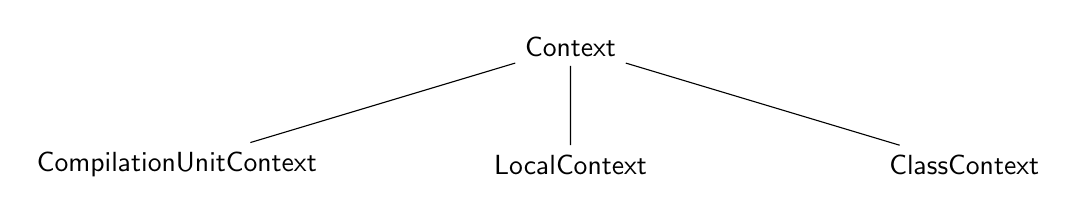
\begin{tikzpicture}[level/.style={sibling distance = 5cm}]
        \node { Context } 
        child{ node {CompilationUnitContext} }
        child{ node {LocalContext} }
        child{ node {ClassContext} };

    \end{tikzpicture}
    \caption{Context tree}
\end{figure}

Dans chacun des contextes associés aux méthodes de classes, on associe
un champ \textit{surrounding context} qui pointe vers le contexte
englobant le bloc correspondant. 

\paragraph{Contexts}
A chaque point d'execution, la table des symbols ressemble à une \textbf{stack
de context} : 

\begin{figure}[!h]
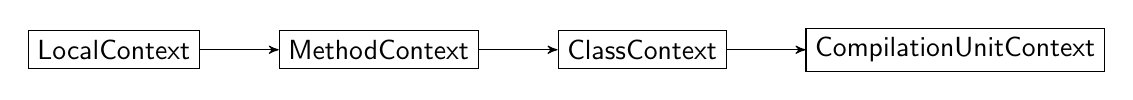
\begin{tikzpicture}
	\node[draw, shape=rectangle] (A) {LocalContext};
    \node[draw, shape=rectangle] (B) [right=of A] {MethodContext};
    \node[draw, shape=rectangle] (C) [right=of B] {ClassContext};
    \node[draw, shape=rectangle] (D) [right=of C] {CompilationUnitContext};
	\path[->] (A) edge (B)
              (B) edge (C)
              (C) edge (D);
\end{tikzpicture}
\caption{Stack context at time t}
\end{figure}

Durant l'analyse, quand le compilateur rencontre une \textbf{variable} il regarde à
cette variable dans la table des symbols en commencant par le \texttt{localContext}.

\begin{itemize}
    \item \texttt{CompilationUnitContext} : scope du programme 
        entier et contient un mapping des noms vers les \textbf{types}:
        \begin{enumerate}
            \item Les type implicits (java.lang.Object, java.lang.String,\ldots)
            \item Les types importés
            \item Les types introduit dans la déclaration de classe
        \end{enumerate}
    \item \texttt{ClassContext} : scope d'une classe et ne contient pas
        de mapping. (Constructor, methodes et champs sont enregistré dans l'objet
        Class)
    \item \texttt{MethodContext} : scope d'une méthode dont les paramètres
        sont déclarés dedans
    \item \texttt{LocalContext} : scope d'un block (\{ \}) contenant les variables locales
\end{itemize}


\begin{figure}[!h]
    \includegraphics[width=10cm]{img/structure-context.png}
    \caption{Structure d'un context}
\end{figure}

\paragraph{Idefns} est un type d'interface pour la définition de la 
table des symboles.

Deux types de Idefns dans les entrées de la table:
\begin{itemize}
    \item \texttt{TypeNameDefn} qui encapsule juste un type
    \item \texttt{LocalVariableDefs} qui défini une variable locale en
        encapsulant son nom, type et un offset dans la frame stack.
\end{itemize}


\begin{figure}
\begin{tabular}{l}
    \includegraphics[height=19cm]{img/AST-context.png}
\\
\begin{lstlisting}
package pass;
import java.lang.System;

public class Factorial {
    public static int factorial(int n) {
        if (n <= 0) return 1;
        else return n * factorial(n - 1);
    }
    public static void main(String[] args) {
        int x = n;
        System.out.println(x + "! = " + factorial(x));
    }
    static int n = 5;
}
\end{lstlisting}
\end{tabular}
\caption{Example AST with context }
\end{figure}

\subsubsection{Finding Method and Field Names in Type Objects}
\todo{LN}

\subsection{Two phase analysis}

L'analyse sémantique besoin de deux traversés de l'AST car des classes et
méthodes peuvent être déclarées après une référence. 

Globalement, \textbf{preAnalyze()} fait ComputationUnitcontext et ClassContext 
ainsi que les informations à propose des types importés/déclaré.
\textbf{analyze()} fait MethodContext et LocalContext, continue la création
des tables de symbol, réécrit l'arbre et fait plusieurs checking.

\subsection{Pre-Analysis of j-\-- program}

\texttt{PreAnalyze()} va:
\begin{itemize}
    \item déclarer les types importés (\texttt{JCompilationUnit} level)
    \item déclarer les class définies par l'user (\texttt{JClassDeclaration} level)
    \item déclarer des champs (\texttt{JFieldDeclaration} level)
    \item déclarer les méthodes (\texttt{JMethodDeclaration} et
        \texttt{JConstructorDeclaration} level)
\end{itemize}

\subsubsection{\texttt{JCompilationUnit.preAnalyse(Context c)}}
\begin{itemize}
    \item Créer le \texttt{CompilationUnitContext}
    \item Déclarer les types implicites \texttt{java.lang.String} 
        et \texttt{java.lang.Object}
    \item Déclarer les types importés
    \item Déclarer les types définis par les déclarations de classe
    \item Invoquer \texttt{preAnalyze()} pour chacun des déclarations
        de type dans la Compilation Unit
\end{itemize}

\subsubsection{\texttt{JClassDeclaration.preAnalyse(Context c)}}
\begin{itemize}
    \item Créer le \textit{Class context} avec \texttt{surroundingContext} 
        qui pointe vers \texttt{CompilationUnitContext}
	\item Résoudre le type \texttt{super} de la classe (check si on n'étend
        pas un class \textit{final})
	\item Créer le \texttt{CLEmitter} associé et y ajoute le class header,
	    le nom et tout les modifications
	\item Invoquer \texttt{preAnalyze} sur les membres de la classe
	\item Rajouter un constructeur explicite s'il n'y a pas
	\item Produire le \textit{Class object}.
\end{itemize}

\subsubsection{\texttt{JMethodDeclaration.preAnalyse(Context c, CLEmitter cle)}}
\begin{itemize}
	\item Résoud les types des paramètres et du \texttt{return}
	\item Vérifie si l'\textit{abstract modifier} est propre

    \item Calcule du descripteur de méthode (codification de la
    signature en string)

        (\texttt{(I)I}: consomme un \texttt{int}, renvoie un
        \texttt{int} ; ([L\texttt{java.lang.String;}])V : prend une
        liste ([]) de strings (L\texttt{java.lang.String;}), revoie
        \texttt{void})
    \item Appelle \texttt{partialCodeGen()} pour générer le code
        de la méthode sans le corp pour que l'objet class ait au-moins les
        informations de l'interface des méthodes (paramètre et le type du
        \texttt{return})
\end{itemize}

\subsubsection{\texttt{JFieldDeclaration.preAnalyse(Context c, CLEmitter cle)}}
\begin{itemize}
	\item Vérifie qu'un champs n'est pas déclaré \texttt{abstract}
	\item Résoud le type du champ
	\item Génère le code bytestream pour la JVM pour la déclaration des champs
\end{itemize}

\subsubsection{Symbol Table built by \texttt{preAnalyse()}}

L'étape de pré-analyse ne déclare aucune variable locale. On a donc
un arbre partiel qui est construit.

%TODO: image?

\subsection{Analayse of j-\-- programs}
Lors de l'analyse, on va effectuer une discrete analyze recursive:

\begin{itemize}
    \item Réécriture de champs et d'initialisation de variables locales
        comme des assignements de variables normales
    \item Déclaration des paramètre formet et des variables locales
    \item Allocation des ressources sur la stack frame
    \item Calcul des types des expressions
    \item Reclassification des noms ambigus
    \item Modification de l'arbre
\end{itemize}


\subsubsection{\texttt{JCompilationUnit.analyse(Context c)}}
Appelle analyze() pour descendre dans l'arbre pour chaque type
de déclaration.

\subsubsection{\texttt{JClassDeclaration.analyse(Context c)}}
Après avoir fait l'analyze() pour chaque field, 
il copie l'initialisation des fields dans son node. 

Il va aussi les séparer en deux : \texttt{staticFieldInitializations}
et \texttt{instanceFieldInitializations}.

\subsubsection{\texttt{JFieldDeclaration.analyse(Context c)}}

Récrit le field initialisé comme un assignement explicit stocké dans
la liste d'initialisation. 

\subsubsection{\texttt{JMethodDeclaration.analyse()}}

\begin{enumerate}
    \item Crée un \textbf{MethodContext} dont \texttt{surroundingContext}
        pointe vers le \texttt{ClassContext} précédant
    \item Le premier stack frame offset  =  0.

        (0 is allocate for \texttt{this} for a instance method)
    \item Les paramètres sont déclaré comme des variables locales
        et alloué sur des offsets consécutif
    \item Il analyse le corps de la méthode comme un context différent.
\end{enumerate}


\paragraph{Stack-frame method}
Nous avons besoin de calculer les offsets de tout les paramètres
ainsi que des variables local pour savoir l'espace nécessaire à
la méthode.

\subsubsection{\texttt{JBlock.analyse()}}

\begin{enumerate}
    \item Crée un nouveau \texttt{LocalContext} dont \texttt{surroundingContext}
        pointe vers le \texttt{MethodContext} précédent et le \textbf{newtOffset} 
        est copié du précédent context.
    \item Analyze son body et chaque \texttt{JVariableDeclarations} declare
        sa variable dans le \texttt{LocalContext} du step 1
\end{enumerate}


\subsubsection{Rewriting a field}

\begin{figure}[!h]
    \includegraphics[width=15cm]{img/field-init.png}
    \caption{Rewriting a field Initialization.
JClassDeclaration (c) et JFieldDeclaration (b) analyse}
\end{figure}

\subsubsection{Method context and local context}

\begin{figure}[!h]
\begin{tabular}{m{6cm}m{4cm}m{4cm}}
\begin{lstlisting}
public class Locals {   
    public int foo(int t, String u) {   
        int v = u.length(); 
        {   
            int w = v + 5, x = w + 7;   
            v = w + x;  
        }   
        {   
            int y = 3;  
            int z = v + y;  
            t = t + y + z;  
        }   
        return t + v;   
    }   
}
\end{lstlisting}
&
    \includegraphics[width=4cm]{img/method-context1.png}
&
    \includegraphics[width=4cm]{img/method-context2.png}
\end{tabular}
\caption{Example method context and local context }
\end{figure}


\subsubsection{Analysing local variable declaration and their initialization}

Avant d'effectuer la méthode analyze(), l'AST contient uniquement les 
\texttt{JVariableDeclarator}.

L'analyse va :
\begin{itemize}
    \item Créer une \texttt{JVariableDefns} avec l'offset de la stack-frame
        correspondant
    \item Vérifié que la variable déclaré n'a pas un nom déja existant
    \item Déclaré la variable dans le \texttt{LocalContext}
    \item Réécrire tout les initialization comme des assignements
        explicits
\end{itemize}

\begin{figure}[!h]
    \includegraphics[width=\linewidth]{img/analysis-variable.png}
    \caption{Analysis variable initialization}
\end{figure}

\subsubsection{Simple variable}

\begin{itemize}
    \item Recherche dans la table des symbols la variable et récupère
        son \texttt{LocalVariableDefn}
    \item Enregistre le \texttt{LocalVariableDefn} pour son utilisation
        dans le code generation et copie le Type
\end{itemize}

\begin{figure}[!h]
    \centering
    \includegraphics[width=10cm]{img/simple-variable.png}
    \caption{Analysis simple variable}
\end{figure}

\paragraph{Note: } Une variable peut représenter un field d'une classe, 
dans ce cas la variable est analyser différement.

\begin{figure}[!h]
    \includegraphics[width=\linewidth]{img/variable-field.png}
    \caption{Analysis d'un field}
\end{figure}

\subsubsection{Field selection and message expression}
%TODO : page 29


\subsubsection{Typing Expressions and Enforcing the Type Rules}
%TODO

\subsubsection{Cast operation}
%TODO

\subsection{The Visitor Pattern and the AST Traversal Mechanism}
%TODO


\subsection{Visitor Pattern and the AST traversal Mechanism}

\section{Chapitre 5 : JVM and Bytecode}

\subsection{Introduction}

Une machine virtuelle est un programme implémentant une machine 
qui exécute un programe comme une machine physique.

\begin{figure}[!h]
    \centering
    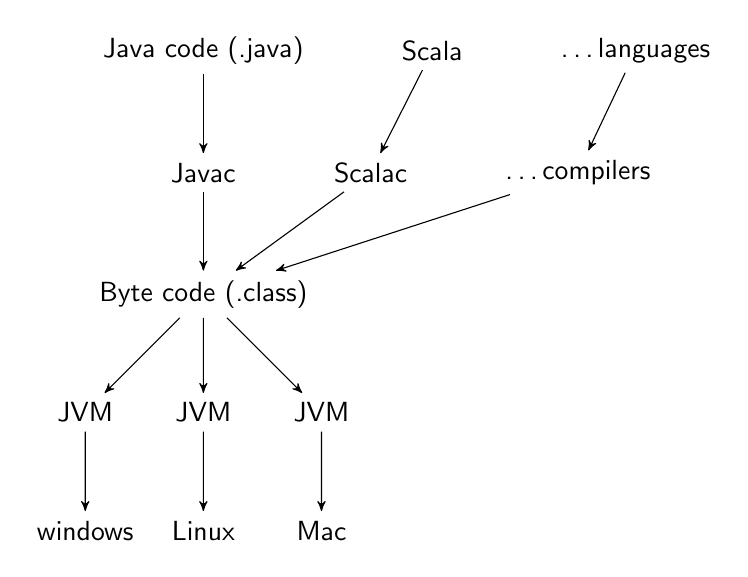
\begin{tikzpicture}[->]
        \node (A) { Byte code (.class) } 
        child{ node {JVM} child{ node {windows}} }
        child{ node {JVM} child{ node {Linux}} }
        child{ node {JVM} child{ node {Mac}} };

        \node (B) [above= of A] {Javac};
        \node (C) [above= of B] {Java code (.java)};

        \node (D) [right= of B] {Scalac};
        \node (E) [right= of C] {Scala};

        \node (F) [right= of D] {\ldots compilers};
        \node (G) [right= of E] {\ldots languages};

        \path[->] (C) edge (B)
                  (B) edge (A)
                  (E) edge (D)
                  (D) edge (A)
                  (G) edge (F)
                  (F) edge (A);
    \end{tikzpicture}
    \caption{JVM}
\end{figure}

D'autres language choisissent de rejoindre la JVM car c'est facile de générer
le code et le byte code est compacte, le code est sur une architecture indépendante
et donc compatible et finalement JVM est efficace et très testé!


\begin{tabular}{m{4.5cm}m{8cm}}
Une instruction \textbf{bytecode} = 
&
\begin{itemize}
    \item Un byte \textbf{opcode}
    \item Un nombre variable d'argument
    \item Offset ou pointeur vers la Constant pool
\end{itemize}
\end{tabular}

Une instuction byte code consumme et produit certain élément de la stack.
Constantes, locals et les éléments de la stack sont typé (adresse ou type
primitifs).

\begin{tabular}{m{4.5cm}m{8cm}}
Un fichier \textbf{.class} = 
&
\begin{itemize}
    \item Magic number (0xCAFEBABE)
    \item Version
    \item Constant pool
    \item Access flag
    \item This class
    \item Super class 
    \item Interfaces
    \item Fields
    \item Methods
    \item Atrributes
\end{itemize}
\end{tabular}

\subsection{Components}

\begin{itemize}
    \item Stack par thread : stocke les stack frames
    \item Heap : mémoire alloué dynamiquement
    \item Constant pool : stocke les constantes et les références
        vers les champs/méthodes
    \item Code segment : stocke code du programme (JVM instruction)
    \item Counter du programme par thread : contient l'addresse de la prochaine instruction
\end{itemize}

\subsection{Stack}

JVM a décidé d'utiliser une stack machine car cela réduit la taille
du byte-code et surtout toutes les opérations travailles sur peu d'élément
au dessus de la stack!

\begin{center}
(\textit{Pour une operation de division d'entier, la machine RISC à
32 registres on a besoin $32*31$ différents opcode (pour chaque paire
possible de registre), alors que la stacke machine n'a besoin que de 1
opcode puisqu'il travaille toujours sur la deux éléments en haut de la
stack})
\end{center}

\subsubsection{Stack loading process}

Les classes (dont le nom doit correspondre avec celui du fichier) sont
chargées de manière \textit{lazy} lors du premier accès, juste après
les super-classes dont elles dépendent. Ensuite le byte-code est vérifié,
les fiels static sont alloué et recoivent leur valeur par défault. Enfin, 
les initialiseur static sont exécuté.

\subsubsection{Frame}
Une nouvelle frame est créé et push sur la stack pour chaque appel
de méhtode. Les stacks sont ensuite pop lorsque la méthode se termine
normalement ou si une exception est \textit{throw}.

\begin{tabular}{m{2.5cm}m{9cm}m{3cm}}
Une frame = 
&
\begin{itemize}
    \item Un tableau de variable locale
    \item Une valeur de retour
    \item Operand stack
    \item Référence vers le \texttt{runtime constant pool} pour la
        classe de la méthode courante.
\end{itemize}
&
\includegraphics[width=3cm]{img/frame.png}
\end{tabular}

\subsubsection{Operand stack}

Appliquer des opérations se fait toujours sur les deux éléments
en haut de la stack. 

\begin{figure}[!h]
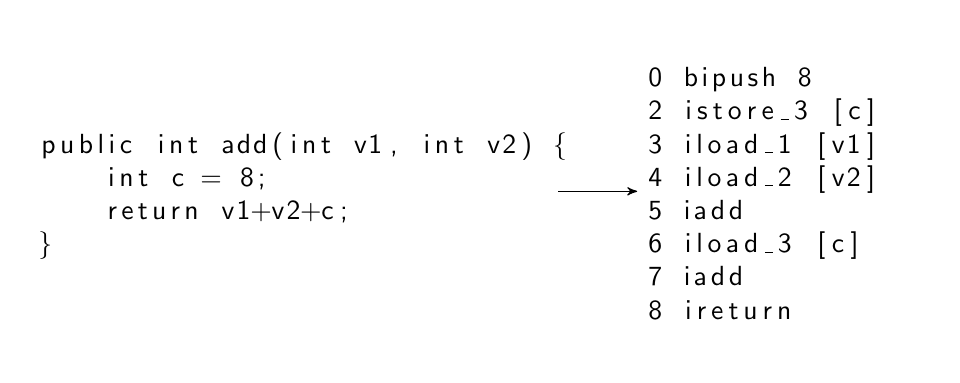
\begin{tikzpicture}
    \node[text width=6.5cm,align=center] (A) 
    {{\begin{lstlisting}
public int add(int v1, int v2) {
    int c = 8;
    return v1+v2+c;
}
\end{lstlisting}}};

\node[text width=3.5cm,align=center] (B) [right= of A] 
    {{\begin{lstlisting}
0 bipush 8
2 istore_3 [c]
3 iload_1 [v1]
4 iload_2 [v2]
5 iadd
6 iload_3 [c]
7 iadd
8 ireturn
\end{lstlisting}}};

	\path[->] (A) edge (B);
\end{tikzpicture}
\caption{Exemple d'utilisation des opérations de stack}
\end{figure}


\subsection{JVM instruction}

\paragraph{Arithmetic}
\texttt{ineg, i2c, iadd, isub, imul, idiv, irem, iinc k i}

\paragraph{Branch}
\texttt{goto L, ifeq L, ifne L, ifnull L, ifnonnull L} : compare
l'élément au top de la stack par rapport à 0.

\texttt{if\_icmpeq L, if\_icmpne L, if\_icmplt L, if\_icmple L,
if\_acmpeq L, if\_acpmne L, if\_icmgt, if\_icmpge} : compare les 2
éléments au top de la stack

\paragraph{Constant loading}
\texttt{iconst\_0, ..., iconst\_5, aconst\_null, ldc i, lds string}.

\paragraph{Field}
\texttt{getfield f sig, putfield f sig, getstatic f sig, putstatic f sig}

\paragraph{Stack}
\texttt{dup, pop, swap, nop, dup\_x1, dup\_x2}

\paragraph{Class}
\texttt{new C, instanceof C, checkcast C}

\paragraph{Méthode}
\texttt{invokestatic name sig, invokevirtual name sig, ireturn, areturn, return}


\subsection{Verification}


\section{Chapitre : Garbage Collection} \todo{quel chapitre?} %LN


Une première manière de manager la mémoire est de manière explicit (malloc/free). Plusieurs désaventage: peut mener à bcp d'erreur (double free, seg fault,...), programmation modulaire bcp plus complexe (il faut se mettre d'accord sur qui free, qui malloc,...).

L'automatisation permet de donner l'illusion d'avoir une infinité de mémoire. Le programmeur ne doit également plus penser à cela. Cela retire également un tas de bugs.


\subsection{Reference Counting}

Chaque objet retient le nombre de réference vers lui-même, incrémentation/décrémentation à chaque création/destruction de référence. Lorsque le compte tombe à 0, suppression de l'objet.

Cette méthode est rapide, sûre et marche dans la plupart des cas (si il y a des références circulaire (A ref B et B ref A), ca ne marche pas).

\subsection{Mark \& Sweep}

Phase 1 : Mark : on démare de root, on trace l'object graph en marquant tout les objets atteints.

Phase 2 : Sweep : on itère sur tout les objets du heap, on supprime les objets non marqué et on clear les marks.

On peut le faire en Depht-first Search (avec ou sans récursion) ou alors en pointer reverse.

Le cout peut être très élevé si il y a peu à jetter. Si plus de 50\% de la heap est concervée, on augmente la taille de la heap.

L'allocation de donnée dans le heap se fait par :
Lorsqu'un objet demande un chunk, on peut donner n'importe quel block de taille >= celle demandée. C'est plus efficace de maintenir des listes des blocks disponible par taille.


Le mark and Sweep permet de gerer les cycles. Par contre, il peut y avoir des problème de fragmentation et un cout d'allocation grand.


\subsection{Copying collection : Cheney algorithm}

On splitte la heap en 2 : from-space et to-space.

Initialement tout les chunck utilisé sont dans le from-space. Au lieu de marquer les chuncks utilisés, on les place dans le to-space. Tout en maintenant à l'ancien emplacement une référence vers le nouvel emplacement.
On déplace ainsi petit-à-petit en suivant les liens. Lorsque l'algo est fini, on inverse les utilisations des deux espaces (from devient to et to deviens from).

Les aventages sont : facile d'allouer de la mémoire (à la fin), pas de fragmentation (compactage automatique), le temps est proportionnel au nombre d'objets vivants. Par contre, il faut le double d'espace mémoire.

\subsection{Generational collection}

On ne fait du tris que dans les objets concidéré comme "jeune", c'est à dire lorsqu'ils ont survécu à plusieurs passage du garbage collector. On a alors une siscion dans la mémoire entre jeune et vieux. Lorsqu'un objet devient vieux, il est déplacé dans la partie vieux.


\section{DSL \& Scala} % Alex

\subsection{Les constructeurs}

En scala, un constructeur "simple" n'a pas besoin d'être défini.

Exemple :

\begin{lstlisting}
class vehicle(name: String, price:Int) {

}

var car = new vehicle("Ferrari", 100000);
\end{lstlisting}

Il est également possible de définir un constructeur "custom" de cette façon là :

\begin{lstlisting}
class vehicle(name: String, price:Int) {

	def this(name: String) = {
		this(name, 10)
	}
}
\end{lstlisting}

\subsection{Les variables}

Deux mots-clefs permettent de définir des variables en Scala : \texttt{val} et \texttt{var}. La différence entre les deux est que les valeurs associées au "vars"
peuvent être modifiées alors que pour les "vals", une seule assignation est possible.

\begin{lstlisting}
var jizz = "jizz"
jizz = "baufays" //Autorise

val poulpe = "poulpy"
poulpe = "manteau louche" //INTERDIT !
\end{lstlisting}

A noter qu'il n'est pas n"cessaire d'écrire le type. Cependant, on peut le faire :

\begin{lstlisting}
val answer: Int = 42 
\end{lstlisting}

\subsection{pure OO}

En Scala, tout est un objet (pas de type primitif). Ainsi, chaque opération est un appel de méthode. de ce fait, "1 + 2" peut s'écrire "1.+(2)".

\subsection{Fonction anonymes}

\begin{lstlisting}
val plusOne = (x:Int) => x+1
plusOne(5) // va retourner 6
\end{lstlisting}

\subsection{closure}

\begin{lstlisting}
//	plusFoo	can reference any values/variables in scope	

var foo = 1
val plusFoo = (x:Int) => x+foo

plusFoo(5) //return 6

foo = 5
plusFoo(5) //now return 10
\end{lstlisting}

\subsection{Higher order function}

Deux choses importantes :

1. l'utilisation de \_ :

\begin{lstlisting}
val nums = List(1,2,3)

nums.exists(_ == 2) //return true
\end{lstlisting}

2. une fonction peut prendre une autre fonction en paramètre.

\subsection{classes}

\subsubsection{object}

Les \texttt{object} sont comme des classes statiques. Donc :

\begin{lstlisting}
object Test extends App
\end{lstlisting}

représente la déclaration d'une classe anonyme qui étend App ainsi que la création d'une unique instance "Test" de cette classe anonyme.\\
A noter que "App" est utilisé comme la classe main en Java.\\
A noter également que les méthodes définies à l'intérieur d'un object sont des méthodes statiques, au sens \#Java8 du terme.

\subsubsection{getters and setters}

Ils n'esistent pas en Scala. Il suffit de faire comme si on accédait a une champ en Java. "nomDeLaClasse.Champ = 'Hélène roule en tracteur'".

\subsubsection{companion object and apply}

Un objet compagnon est un objet qui porte le même nom que la classe qu'il accompagne.
La spécificité étant que la classe peut accéder au membres privés de l'objet et vice versa.

La méthode "apply" est une méthode qui agit un peu comme un constructeur pour les objects et qui peut être utilisée avec les classes comme sucre syntaxique :

\begin{lstlisting}
//Exemple 1

class Calculator(brand: String) {	
	def add(m: Int, n: Int): Int = m + n	
}

object Calculator {	
	def apply(brand: String) = new Calculator(brand)	
}

object Test extends App {	
	
val c1 = new Calculator("HP") //sucre syntaxique pour Calculator.apply("HP")
val c2 = Calculator("HP") // TODO : Different de celui du dessus ???
}


//Exemple 2

class Test(n: Int) {
	def apply(m: Int) = {
    	return m+n
    }
}

object Main extends App {
	val t = Test(1)
    println(t(2)) // va imprimer '3'
}
\end{lstlisting}

\subsubsection{operator overload}

Il suffit de réecrire une méthode avec le même nom...

\subsection{Mutability}

\todo{What is this fuk ? En quoi c'est cool/pas cool ? \#poulpe}

\subsection{Null and options}

Null, c'est nul ! Difficle à gérer. Si une variable peut être nulle, il faut checker, sinon risque de \texttt{NullPointerException}.

A la place, il faut utiliser le type \texttt{Option[T]}. Selon le cas, cela va nous renvoyer \texttt{Some(x)} si x existe, \texttt{None} dans l'autre cas.

\subsection{Currying (et safraning, paprikaning, etc.)}

On peut définir plus qu'une séquence d'arguments.

\begin{lstlisting}
def add(a)(b) = a+b
add(1)(2)
\end{lstlisting}

\subsection{Call by name}

En général, par exemple en \#Java8\footnote{pour les intimes...}, on fait du call by value. C'est à dire que les arguments d'une fonction seront toujours évalué avant l'exécution de la fonction. De ce fait, on connait la valeur de ces arguments. Par exemple, si un des argument est "2+2", on l'évaluera à "4"
avant de lancer l'exécution de la fonction.

Dans le call by name, on peut utiliser des fonctions comme argument, et celles-ci ne seront évaluées que lorsque l'on en aura besoin (un peu comme le "lazy" qu'on a vu en OZ).

L'avantage du by value est que la fonction utilisée en argument n'est évaluée qu'une seule foi. L'avantage du by name est que si on a pas besoin d'évaluer la fonction on ne le fera pas.

Les deux méthodes sont équivalentes dans le cas de fonctions pures et si les exécutions terminent. Par exemple :

\begin{lstlisting}
object Test {
   def main(args: Array[String]) {
        delayed(time());
   }

   def time() = {
      println("Getting time in nano seconds")
      System.nanoTime
   }
   def delayed( t: => Long ) = {
      println("In delayed method")
      println("Param: " + t) //1
      wait(5000)
      println("Param: " + t) //2
   }
}
\end{lstlisting}

Ici, si on fait du by value, les deux print imprimeront la même chose. Par contre, dans le cas du by name, la fonction sera recalculée et on aura deux valeur différente à imprimer. \todo{correct ?}\\

Notons qu'en Scala, l'utilisation du by value est celle pas défaut. Si on veut du by name, on doit ajouter "=>" devant le type de l'argument.

\subsection{implicit conversion}

Permet de convertir automatiquement un type en un autre pour pouvoir appliquer certaines opérations. Exemple :

\begin{lstlisting}
import ComplexImplicits._	
	
object ComplexImplicits {	
	implicit def Double2Complex(value : Double) = new Complex(value,0.0) 	
	}	

object MyComplex extends App {	
	
	val d = Complex(1)(2)	
	val e = 1+d	//Ici, le Int 1 va automatiquement etre converti en Complex
    			//via la methode Double2Complex
}
\end{lstlisting}

\subsection{implicit classes}

\todo{heu ... ?}

\subsection{implicit parameters}

En gros, c'est une loucherie qui permet de remplacer automatiquement un argument d'une fonction si on apelle la fonction sans cet argument. Après...

\todo{A completer}

\subsection{Traits}

Les traits sont à la frontière entre les interfaces et les classes abstraites.

En effet, le trait est plus riche que l'interface en ce sens qu'elle peut contenir une implémentation. En outre, le trait diffère de la classe abstraite par le fait que son constructeur ne peut contenir aucun paramètre et, il est lié dynamiquement, permettant un héritage multiple.

Ce n'est pas un objet (on ne peut pas l'instancier).
C'est un truc entre les interfaces et les classe abstraite. Comme une interface, c'est implémenté par une classe et cela contient un certain nombre de signatures de méthodes que la classe devra implémenter. Mais comme une classe abstraite, il y a un certain nombre de méthodes déjà implémentées. Par contre un trait ne peut pas être instancié.

Exemple :

\begin{lstlisting}
trait Comp {

def < (that : A): Boolean

def > (that : A): Boolean = {...}
def >= (that : A): Boolean = {...}
...

}
\end{lstlisting}

\subsection {Monads}
Il s'agit d'une structure e donnée qui défini à la fois \texttt{map} (prend un iterable et applique la fonction passée en argument) et \texttt{flatMap} (idem que map mais avec un flatten en plus: \texttt{[1, [2]]} $\Rightarrow$ \texttt{[1, 2]}: on aura plus qu'une seule liste à la fin) et \texttt{Unit}.\\

Tous les types \texttt{M[T]} donc en gros des listes de \texttt{T} (structure de données génériques) et qui ont deux opérations spéciales: \texttt{flatMap} et \texttt{unit}
\begin{itemize}
	\item[\texttt{flatMap}]: prend une fonction en argument et l'applique à tous les éléments de la structure et va faire un flatten (\texttt{[1, [2]]} $\Rightarrow$ \texttt{[1, 2]}: on aura plus qu'une seule liste à la fin)
    \item[\texttt{unit}]: va prendre une valeur en argument (du type générique de la structure) et va créer une structure avec cette élément dedans. Ex: \texttt{List(x)}: on aura une liste avec \texttt{x} comme premier élément de la structure.
\end{itemize}


\subsection{Yield}
Va faire une espère de link dans le type du premier du for:
\begin{lstlisting}
val A = Array(1,2)	
val B = List(1,2)
for (i <- A; j <- B) yield (i,j) 	
// Array((1,1),	(1,2), (2,1), (2,2))	
for (i <- B; j <- A) yield (i,j) 	
// List((1,1), (1,2), (2,1), (2,2))
\end{lstlisting}




\chapter{Questions d'exam}

\section{Lexical Anal. IS-IS}

\section{Grammar}

\subsection{Give an example of ambiguity in a real programming language. How is it managed in practice?}
\todo{explain}
\begin{align}
E ::=& E+E & & E ::= TE'\\
E ::=& E\times E & & E' ::=  +TE'\\
E ::=& (E) & &E' ::= \epsilon\\
E ::=& id & & T ::= \times FT'\\
& & & T' ::= \epsilon\\
& & & F ::= id\\
& & & F ::= (E)
\end{align}
À gauche, elle est ambigüe (on peut avoir deux arbres) mais pas à droite ($LL(1)$)

\section{Parsing}

\section{Chapitre 4 : Type checking}

\subsection{Why a two phase analysis ? Describe what each phase does.}

L'analyse sémantique de programmes j-- (et Java) requière deux parcours de l'AST parce qu'un nom de classe ou le nom d'un membre peut être référencé avant qu'il ne soit décllaré dans le code source.

\subsubsection{pre-analyse}

La pré-analyse traverse l'AST moins profondément que l'analyse.
Cependant, elle va suffisamment loin pour :
\begin{itemize}
\item Les déclarations des noms des types importés.
\item Les déclaration des noms des classes définies par l'utilisateur.
\item Les déclarations de champs.
\item Les déclarations de méthodes (incluant leur signature et le type des paramètres).
\end{itemize}

Pour cette raison, \texttt{preAnalyze()} ne doit être défini que pour certains noeuds de l'AST : \texttt{JCompilationUnit, JClassDeclaration, JFieldDeclaration, JMethodDeclaration, JConstructorDeclaration}.

Donc, comme on peut le constater, la phase de pré-analyse ne parcourt pas le corps des méthodes.

\subsubsection{analyse}

Elle s'effectue logiquement après la pré-analyse, et parcourt l'entièreté de l'AST, jusqu'au feuilles.
Elle sert à :
\begin{itemize}
\item Réécrit les initialisations de champs et de variables locales comme des assignements.
\item Déclare les paramètres formels et les variables locales.
\item Alloue des stack frames pour les paramètres formels et les variables locales.
\item Résout le type des expressions et assure les règles de types du langage.
\item Reclassifier les noms ambigus.
\item Faire une partie de "tree surgery".
\end{itemize}

\subsection{When is the final modfifier of classes checked ?}

Dans la méthode \texttt{preAnalyze()} applicable aux noeuds de type \texttt{JClassDeclaration}.

Si une classe est "finale", elle ne peut pas être étendue. On vérifie donc pour chaque classe que le super-type n'est pas final.

\subsection{When is abstract method body checked ?}

Une méthode abstraite possède comme particularité qu'elle ne peut pas avoir de corps.
On vérifie cela dans la méthode \texttt{preAnalyze()} applicable sur les noeuds de type
\texttt{JMethodDeclaration}.

\subsection{Explain memory allocation ? How variable offset are computed ?}

Voir pages 143 à 152 du bouquin. \#JeFaisCommePoulpyPourReseau\\
Mémoire: this, parameters, block (nextOffset + la place en mémoire)

\subsection{Explain how variable shadowing is detected.}

Dans le context de la méthodes, on alloue les stack frames (voir question précédente) au fur et à mesure de l'avancement dans la méthode. Chacune de ses frames contient, entre autre, le nom de la variable. Ce qu'on fait, c'est que dans la méthode \texttt{analyze()} applicable sur les noeuds de type \texttt{JVariableDeclaration}, avant d'ajouter la variable au \texttt{LocalContext}, on fait un lookup dans ce context pour vérifier que le nom n'est pas déjà utilisé. Si c'est le cas, on reporte une erreur ; sinon, on ajoute la variable au context.

\subsection{Explain where type-checking is done ?}

Dans la méthode \texttt{analyze()} applicable sur les noeuds de type \texttt{JVariable}.\\
Surtout pour les check: if avec un boolean, cast correct

\subsection{What do we do for the cast ?}

Ca se fait dans la méthode \texttt{analyze()} pour les noeuds \texttt{JExpression}. On vérifie le type dans lequel on veut
caster l'expression. S'il est valide, alors on crée un \texttt{Converter} qui va être utilisé au moment de la génération de code pour générer le code requis pour le cast. S'il n'y a aucun \texttt{Converter} défini, alors on peut conclure que le cast est invalide.


\end{document}
